% !TEX root=../pldi2019.tex



\section{Semantics}
\label{sec:semantics}

In this section we formalise the semantics of the language constructs described in \cref{sec:language}.
We organize this by following the structure of the language.

Firstly, the task language is embedded in a simply typed lambda calculus.
This requires a specification of the evaluation of terms in the host language, and how it handles the task language.

Secondly, there are two ways to drive evaluation of task expressions, internally by the system itself, and externally by the user.
This is done in two additional semantics, one for the internal normalisation of tasks, and another for the interaction with the end user.

One of our explicit goals is to keep the semantics for evaluation and normalization separate.
This is achieved by letting tasks be values in the host language.

The three main layers of semantics are thus \emph{evaluation}, \emph{normalisation}, and \emph{interaction}.
The semantics, together with \emph{observations}, will be discussed in the following subsections.
\Cref{fig:semantic-functions} shows the relation between the semantics.
It also shows that there are two helper semantics, \emph{handle} and \emph{stride}.

\begin{figure}[h]
  \centering
  \includegraphics[width=\columnwidth,page=5]{figures/drawings-crop.pdf}
  \caption{
    Semantic functions defined in this report and their relation.
  }
  \label{fig:semantic-functions}
\end{figure}

We use the convention that downward arrows are big-step semantics, and rightward arrows are small-step semantics.



\subsection{Evaluating expressions}
\label{sec:evaluation}

The host language evaluates expressions using a big-step semantics.
Evaluating an expression $e$ in state $s$ into a value $v$ in state $s'$ is denoted by $\RelationE$.
To ease reasoning about references, we choose a call-by-value evaluation strategy.

\Cref{fig:value-grammar} shows values with respect to the evaluation semantics.
Tasks are values, and the operands of task constructors are evaluated eagerly.
Exceptions to this are steps and external choice, where some or all of the operands are not evaluated.

\begin{figure}[h]
  \small
  \usemacro{G-Values-Compact}
  \caption{Value grammar} \label{fig:value-grammar}
\end{figure}

The rules to evaluate expressions $e$ do not differ from standard work, except for the task constructs.
The evaluation rules for tasks can be deduced from the value grammar.
They are given in the appendix.



\subsection{Task observations}

% \begin{figure*}[b]
%   \small
%   \usemacro{O-Value-Compact} \hfill \usemacro{O-Failing-Compact} \hfill \usemacro{O-Inputs-Compact}
%   \caption{Values} \label{fig:observation-value}
% \end{figure*}

The normalisation and interaction semantics make use of observations on tasks.
Observations are semantic functions on the syntax tree of tasks.
There are four semantic functions: $\Value$ for the current task value, $\Failing$ to determine if a task fails, $\Inputs$ for the currently accepted input events, and a function for generating user interfaces.
The semantics make use of $\Value$ and $\Failing$, while $\Inputs$ is used for proving safety.
The function for user interfaces is not used by the semantics, but by our implementation.
It is only described in passing here.




\paragraph{Observable values $(\Value)$}

Task values are used by steps to calculate the successor task.
Filled editors are tasks which contain values, as are shared editors.
Unvalued editors do not contain values, neither does the fail task.
These facts propagate through all other task constructors.
The partial function $\Value$ associates a value $v$ to tasks $t$ where possible.
Its definition is given in \cref{fig:observation-value}.

\begin{figure}[h]
  \small
  \usemacro{O-Value}
  \caption{Values} \label{fig:observation-value}
\end{figure}

Internal and external steps do not have an observable value, because calculating the value would require evaluation of the continuation.
Parallel composition only has a value when both branches have values, in which case these values are paired.
Internal choice has a value when one of the branches has a value.
When both branches have a value, it takes the value of the left branch.
External choice does not have a value because it waits for user input.



\paragraph{Failing $(\Failing)$}

In \cref{sub:fail} we introduced $\Fail$ to stand for an impossible task.
Combinations of tasks can also be impossible.
Take for example the parallel composition of two fails ($\Fail \And \Fail$).
This expression is equivalent to $\Fail$, because it can not handle input and can not be further normalized.

This intuition is formalised by the function $\Failing$ in \cref{fig:observation-failing}.
It determines whether a task is impossible.
Such tasks are called \emph{failing}.

\begin{figure}[h]
  \small
  \usemacro{O-Failing}
  \caption{Failing} \label{fig:observation-failing}
\end{figure}

Steps whose left hand sides are failing can never proceed because of the lack of an observable value.
Therefore they are itself failing.
The internal choice of two failing tasks is failing.
External choices let the user pick a side and only then evaluate the corresponding subexpression.
To determine if an external choice is failing, it needs to peek into the future to check if both subexpressions are failing.
Annotations are failing only if the inner task is failing.



\paragraph{User interface}

\TOPHAT is designed such that a user interface can be generated from a task's syntax tree.
A possible graphical user interface is shown in \cref{fig:flight-booking}, where tasks are rendered as \HTML pages.
Editors are rendered as input fields,
external choices are represented by two buttons,
and parallel tasks are rendered side by side.
Steps only show the interface of their left hand side.
In case of an external step they are accompanied by a button.
When the guard condition of a step is not fulfilled, the button is disabled.



\subsection{Normalising tasks}
\label{sec:normalise}

The normalisation semantics is responsible for reducing expressions of type $\Task$ until they are ready to handle input.
It is a big-step semantics, and makes use of evaluation of the host language.
We write $\RelationN$ to describe that
an expression $e$ in state $s$ normalises to task $t$ in state $s'$.

Normalisation rules are given in \cref{fig:normalisation-semantics}.
Both rules ensure that expressions are first evaluated by the host language ($\evaluate$), and then by the stride semantics ($\stride$).
These two actions are repeated until the resulting state and task stabilise.

\begin{figure}[h]
  \small

  \boxed{\RelationN}
  \begin{mathpar}
    \userule{N-Done} \\
    \userule{N-Repeat}
  \end{mathpar}
  \caption{Normalisation semantics} \label{fig:normalisation-semantics}

\end{figure}

The split between striding and normalisation is due to mutable references.
Consider the following example, where $s=\set{l\mapsto\False}$.
\begin{TASK}
  (update l >>= \x:Bool. if x then e else fail) <&> (l := True; edit <<>>)
\end{TASK}
\refrule{S-And} reduces this expression in one step to
\begin{TASK}
  (update l >>= \x:Bool. if x then e else fail) <&> (edit <<>>)
\end{TASK}
with $s'=\set{l\mapsto\True}$.
This expression is not normalised, because the left task can take a step.
The issue here lies in the fact that the right task updates $l$.
To overcome this problem, the \refrule{N-Done} and \refrule{N-Repeat} rules ensure that striding is applied until the state $s$ becomes stable and no further normalisation can take place.

The striding semantics is responsible for reducing internal steps and internal choices.
A stride from task $t$ in state $s$ to $t'$ in state $s'$ is denoted by $\RelationS$.
The rules for striding are given in \cref{fig:striding-semantics}.
Tasks like editors, fail and external choice are not further reduced.
For external choice and parallel there are congruence rules.

\begin{figure}[h]
  \small

  \begin{mathpar}
    \boxed{\RelationS}
  \end{mathpar}

  \paragraph{Step}
  \begin{mathpar}
    \userule{S-ThenStay} \\
    \userule{S-ThenFail} \\
    \userule{S-ThenCont}
  \end{mathpar}

  \paragraph{Choose}
  \begin{mathpar}
    \userule{S-OrLeft} \\
    \userule{S-OrRight} \\
    \userule{S-OrNone}
  \end{mathpar}

  \paragraph{Ready}
  \begin{mathpar}
    \userule{S-Edit} \quad \userule{S-Fill} \qquad \userule{S-Update} \\
    \userule{S-Fail} \quad \userule{S-Xor}
  \end{mathpar}

  \paragraph{Congruence}
  \begin{mathpar}
    \userule{S-Next} \quad
    \userule{S-And} \\
    %\userule{S-Appoint}
    % \userule{S-Eval}
  \end{mathpar}

  \caption{Striding semantics} \label{fig:striding-semantics}
\end{figure}



\paragraph{Principles of stepping}
\label{sub:stepping-principles}

Stepping away from task $t_1$ can only be performed when
$t_1$ has a value: $\Value(t_1) = v_1$.
Only then can a new task $t_2$ be calculated from the expression $e$.
On top of that, $t_2$ must not be failing: $\neg\Failing(t_2)$.

These principles lead to the stepping rules in \cref{fig:striding-semantics}.
\refrule{S-ThenStay} does nothing,
because the lhs does not have a value.
\refrule{S-ThenFail} covers the case that
the lhs has a value but the calculated successor task is failing.
This rule uses the semantics of the host language to evaluate the application $e_2 v_1$.
When all required conditions are fulfilled, \refrule{S-ThenCont} allows stepping to the successor task.



\paragraph{Principles of choosing}
\label{sub:choosing-principles}

Choosing between two tasks $t_1$ and $t_2$ can only be done when
at least one of them has a value: $\Value(t_1) = v_1 \lor \Value(t_2) = v_2$.
When both have a value, the left task is chosen.
When none has a value, none can be chosen.
These principles lead to the rules \refrule{S-OrLeft}, \refrule{S-OrRight}, and \refrule{S-OrNone},
which encode that the choice operator picks the leftmost task that has a value.



\subsection{Handling user inputs}
\label{sec:handling}

The handling semantics is the outermost layer of the stack of semantics.
It is responsible for performing external steps and choices, and for changing the values of editors.
The rules of the interaction semantics are given in \cref{fig:interaction-semantics}.
The semantics is only applicable to normalized $t$.
Sending an input event $i$ to a task $t$ first handles the event and then prepares the resulting task for the next input by normalising it.

\begin{figure}[h]
  \small
  \begin{mathpar}
    \boxed{\RelationI} \\
    \userule{I-Handle}
  \end{mathpar}
  \caption{Interaction semantics} \label{fig:interaction-semantics}
\end{figure}

Handling input is done by the \emph{handling} semantics shown in \cref{fig:handling-semantics}.
It is a small step semantics with labelled transitions.
It takes a task $t$ in a state $s$ and an input $i$, and yields a new task $t'$ in a new state $s'$.
Inputs $i$ are formed according to the grammar in \cref{fig:input-grammar}.

\begin{figure}[h]
  \small
  \usemacro{G-Inputs-Compact}
  \caption{Input grammar} \label{fig:input-grammar}
\end{figure}

% As we already discussed before,
% there are three actions that can be handled by editors:
% \begin{enumerate*}
%   \item filling in an unvalued editor;
%   \item changing the value; or
%   \item clearing the value.
% \end{enumerate*}
% We choose to merge the first two, filling and changing, into one action.
% The value of an editor, empty or not, can be changed to a value $v$ by just sending the value as an action.
% To empty a valued editor, we send the $\Empty$(mpty) action.

% To change values in an editor,
% systems should interact with the user by some kind of interface.
% In a graphical setting,
% we can present the user an input box.
% The user can then change and clear values continuously.
% In a text oriented world,
% we can print out the current value of an editor
% and prompt the user for a new value
% or a command to empty the editor.
% To abstract away from the user interface,
% we introduce an event system.
% It does not matter how these events are sent to the application.
% This can be by pushing a button,
% entering text in an input box,
% committing some text on a command line,
% sending it over a web socket,
% etc.

% In a previous attempt to build a semantics for \TOP,
% \textcite{theses/radboud/VinterHviid18} also used the notion of events.
% However, \citeauthor{theses/radboud/VinterHviid18} made events part of the task layer.
% This means the programmer has access to events using a \texttt{getEvent} function call.
%
% In this work,
% we deviate from above idea.
% We use labeled transitions in the same way as \textcite{school/maktoberdorf/PeytonJones01},
% who gives denotational semantics to the Haskell \IO monad.

\begin{figure}[h]
  \small

  \begin{mathpar}
    \boxed{\RelationH}
  \end{mathpar}

  \paragraph{Editing}
  \begin{mathpar}
    \userule{H-Change} \quad
    \userule{H-Empty} \\
    \userule{H-Fill} \quad
    \userule{H-Update}
  \end{mathpar}

  \paragraph{Continuing}
  \begin{mathpar}
    \userule{H-Next} \\
    \userule{H-PickLeft} \quad
    \userule{H-PickRight}
  \end{mathpar}

  \paragraph{Passing}
  \begin{mathpar}
    \userule{H-PassThen} \quad \userule{H-PassNext} \\
    \userule{H-FirstAnd} \quad \userule{H-SecondAnd} \\
    \userule{H-FirstOr}  \quad \userule{H-SecondOr}\\
  %  \userule{H-Appoint}
  \end{mathpar}

  \caption{Handling semantics} \label{fig:handling-semantics}
\end{figure}

Inputs can be simple actions which interact with editors, external steps and external choices.
Corresponding to \cref{fig:editor-state}, the value of any editor can be changed by sending a new value $v$.
Valued editors can be emptied by sending the special action $\Empty$(mpty).
Note that the conditions to the right of the editing rules take care of typing.
Only when the entered value $v'$ has the same type $\tau$ as the original value $v$ we can change the value of an editor.

To proceed with an external step, users send the $\Continue$(ontinue) action.
As with internal stepping, this is only possible when the lhs has a value and the continuation is not failing.
$\Left$ and $\Right$ are used to pick the left or right option of an external choice.
Inputs $\First$(irst) and $\Second$(econd) are only used to direct inputs to the correct branch of parallel combinations.
Additionally, there are two rules to pass any event on to the left of a step, to be able to reach other nested tasks.
The notable exception is off course $\Continue$, which has to be handled by the external step itself.

In order to know which inputs a task expects, we have constructed a function that calculates a set of all possible inputs that can be handled.
This function called inputs, denoted with $\Inputs$, takes the current normalised expression and state, and returns a set of inputs that can be handled.
The definition of this function is listed in Figure~\ref{fig:observation-input}.

\begin{figure}[h]
  \small
  \usemacro{O-Inputs}
  \caption{Inputs} \label{fig:observation-input}
\end{figure}



\subsection{Implementation}

The semantics have been implemented in the Idris programming language \cite{journals/jfp/Brady13}.
We use techniques presented by \textcite{journals/entcs/JaskelioffGH11}, \textcite{journals/jfp/Swierstra08}, and \textcite{school/maktoberdorf/PeytonJones01}.
Such an implementation increases the confidence in the correctness and completeness of the semantics.
The source code can be found on GitHub.\footnote{\url{http://github.com/XXX/XXX}}
A proof of concept implementation in Haskell is also available, showing that \TOPHAT can be implemented without dependent types.

A command-line interface is part of this implementation.
It prompts users to type input events, which get parsed and processed by the interaction semantics.
